\documentclass[../delivery_hospital_report.tex]{subfiles}
\graphicspath{ {images/}{../images/}{../../images/} }

\begin{document}
\clearpage
\section{Percepção Externa}

A placa de Percepção Externa é a mais complexa dentre todas. Ela foi idealizada, desde da primeira versão do robô hospitalar, para realizar a leitura de todos sensores de distância e de mensurar o estado do robô a partir de um sensor de inércia. Além de claro, como já mencionado antes, enviar e receber informações da placa de controle principal. De maneira geral, ela foi pensando em coletar dados do mundo externo para o robô.

\subsection{Placa}

Como módulo, existem muitas minúcias que precisamos tomar ao projetá-las. A placa de Percepção Externa, para segunda versão do robô hospitalar, com objetivo de evitar problemas e realizar testes, teve duas versões: um protótipo, que já foi finalizado, e uma versão oficial, ainda em desenvolvimento. 

%================================ PERCEPÇÂO PROTOTIPO ========================
\subsubsection{Protótipo}

O protótipo das placas foi refeito duas vezes. Como se trata de uma placa fresada, pode ser refeita no próprio laboratório do professor orientador. A primeira placa não funcionou porque a impressão ficou ruim. O projeto da placa eletrônica, assim como o de todos os módulos, foi dividido em esquemático e Printed Circuit board (PCB)  ou placa de circuito impresso. 

\begin{figure}[!h]
\centering
    \caption{Protótipo placa de Percepção Externa - Esquemático principal }
    \centering % para centralizarmos a figura
    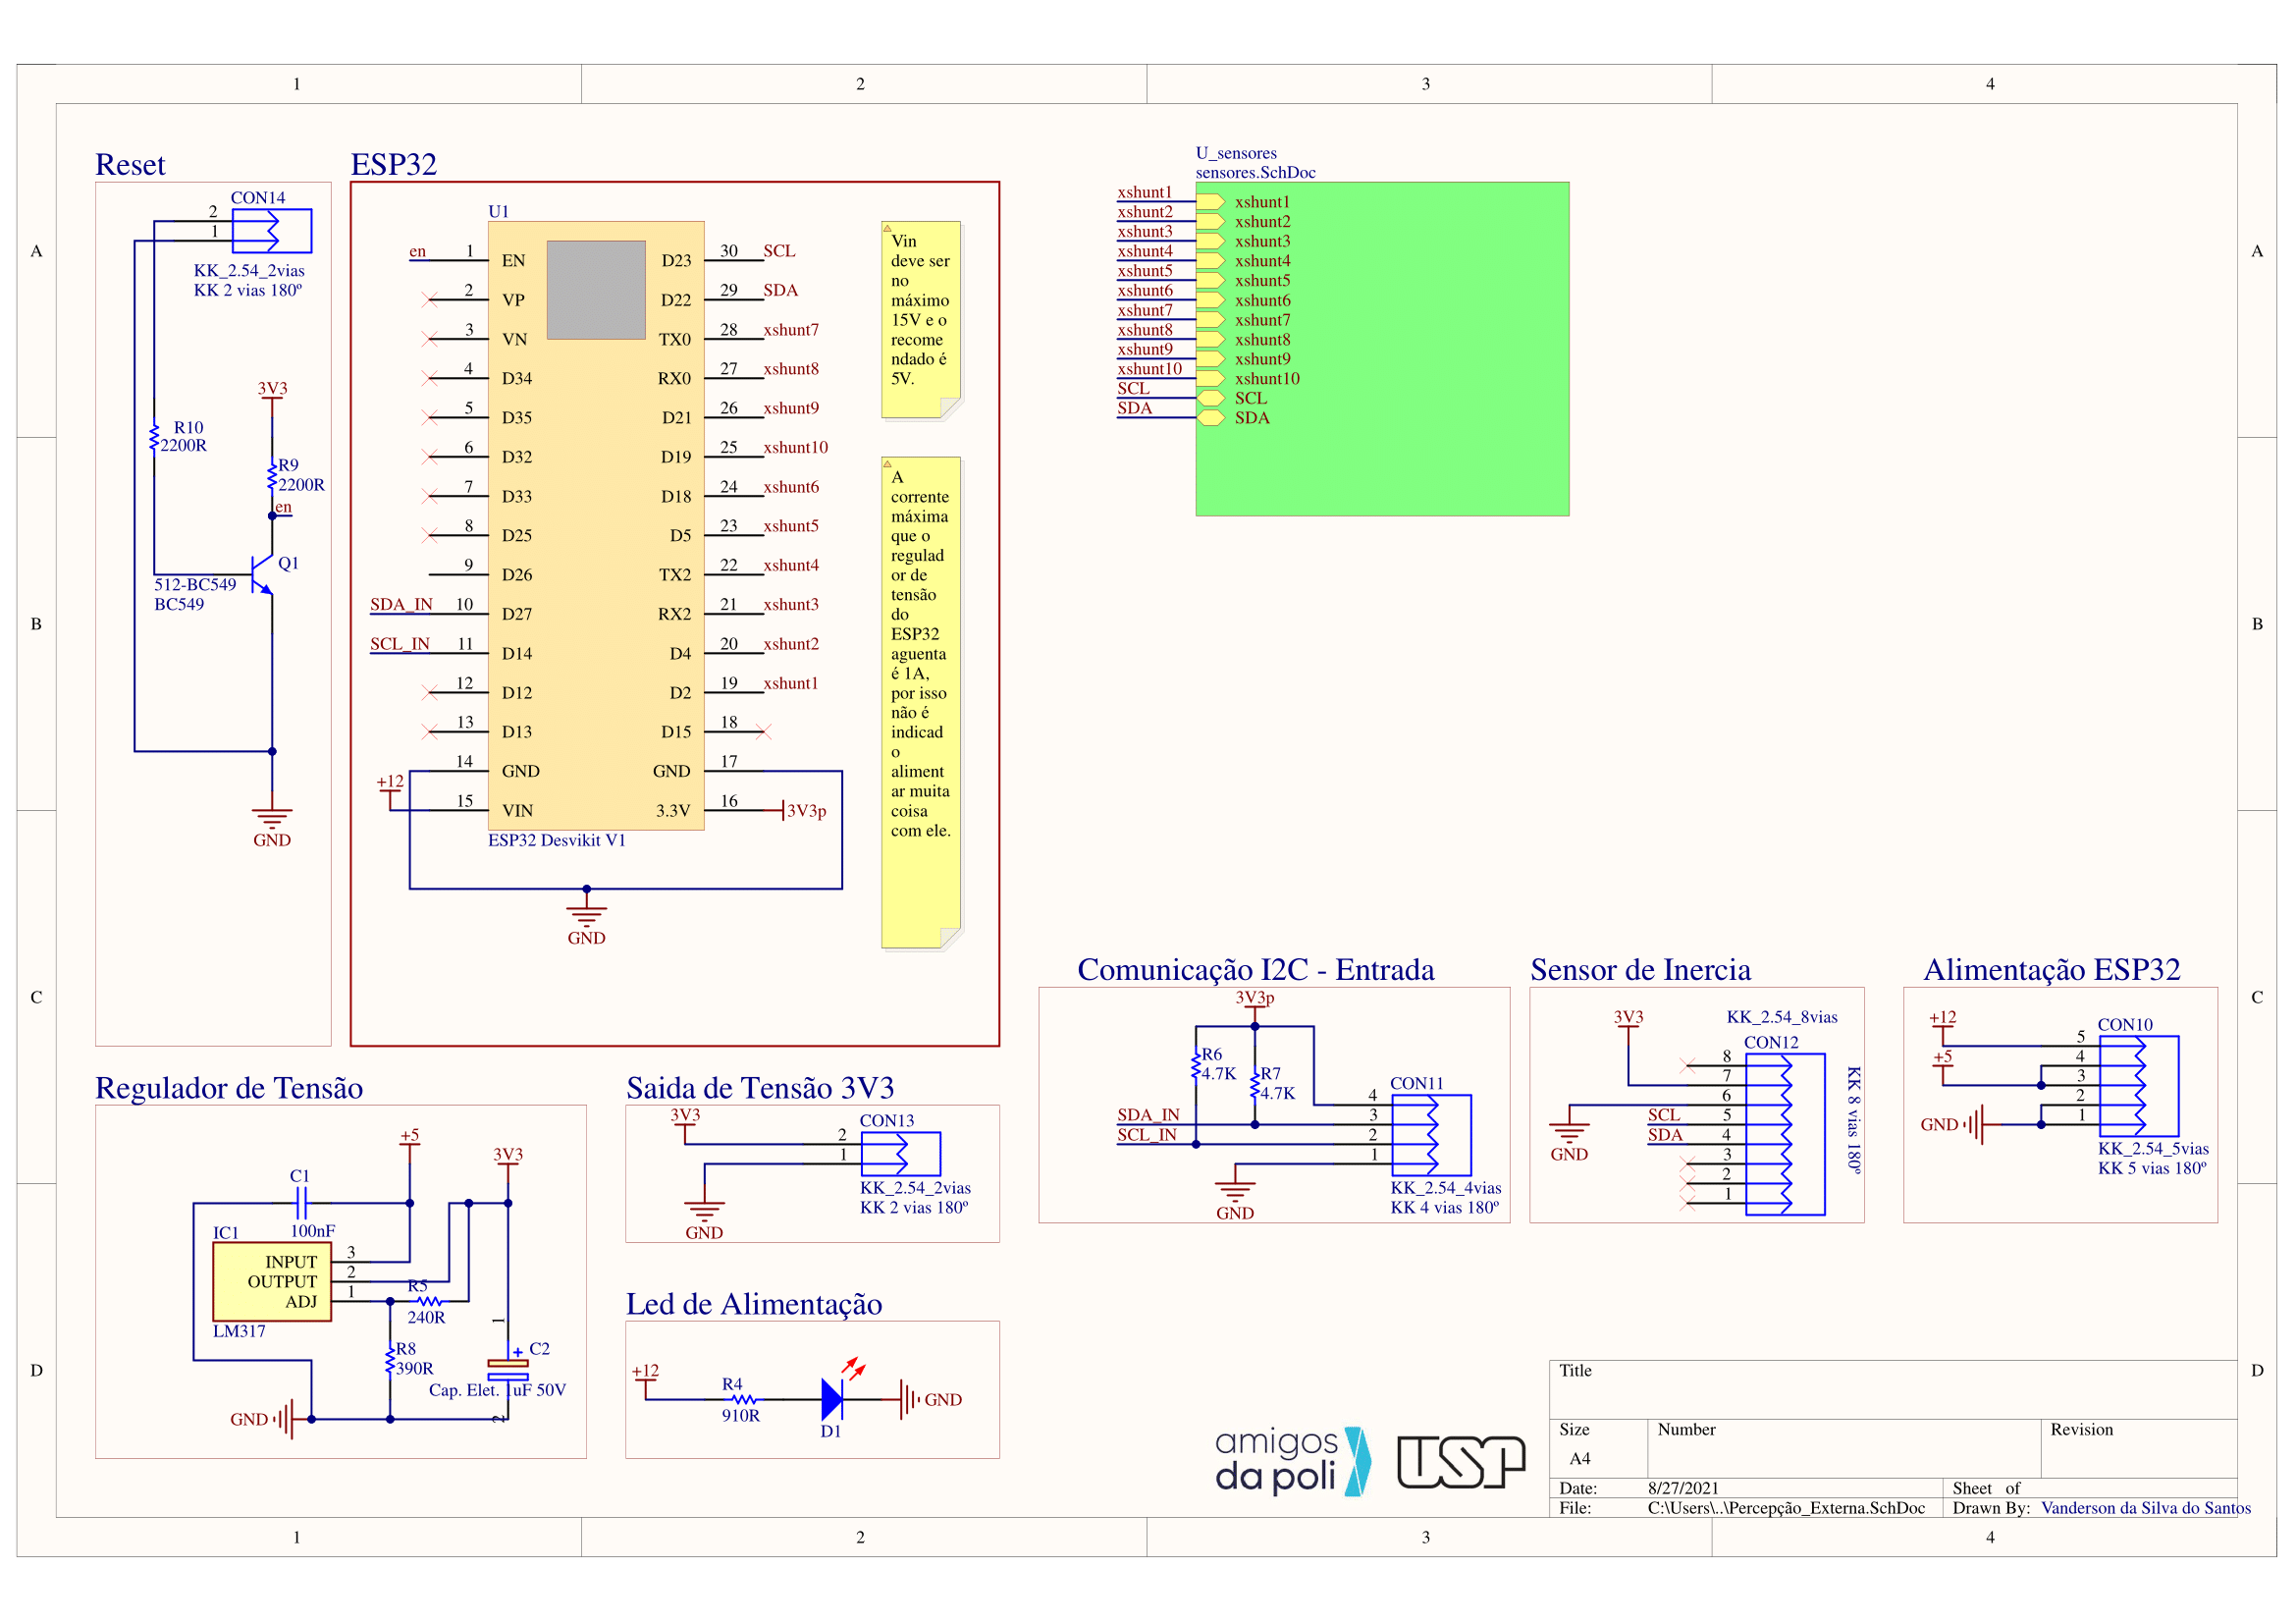
\includegraphics[width=17cm]{modulos/Percepção_Externa-1.png}
    \caption*{Fonte: Elaborado pelo autor no software Altium Design\cite{altium21} }
    \label{Protótipo placa de ## - Esquemático principal}
\end{figure}

Para design do hardware do módulo de controle foi utilizado o CAD e software Altium Designer 21 \cite{altium21} a partir de uma licença estudantil. O projeto completo está disponibilizado em \cite{github_modulos} e todos os componentes usado nesse protótipo podem ser visto na tabela ~\ref{table:Componentes Utilizados na placa de Percepção Externa - Protótipo}.

\begin{table}[!ht]
\caption{Componentes Utilizados na placa de Percepção Externa - Protótipo}
\centering
\begin{adjustbox}{width=\columnwidth,center}
\begin{tabular}{|c|c|c|c|c|}
\hline
Component                     & Description                                                    & Designator                                                    & Footprint                   & Quantity \\ \hline
100nF                       & CAP CER DISK 100NF   50V                                       & C1                                                            & CAP CER DISK 100NF   50V    & 1        \\ \hline
Cap. Elet. 1uF   50V        & Aluminum Organic   Polymer Capacitors 16volts 470uF ESR 10mohm & C2                                                            & Cap. Elet. 470uF 16V        & 1        \\ \hline
KK\_2.54\_6vias             & Conector KK 2.54mm 6   vias                                    & CON1, CON2, CON3,   CON4, CON5, CON6, CON7, CON8, CON9, CON15 & KK\_6vias\_180°             & 10       \\ \hline
KK\_2.54\_5vias             & Conector KK 2.54mm 5   vias                                    & CON10                                                         & KK\_5vias\_180°             & 1        \\ \hline
KK\_2.54\_4vias             & Conector KK 2.54mm 4   vias                                    & CON11                                                         & KK\_4vias\_180°             & 1        \\ \hline
KK\_2.54\_8vias             & Conector KK 2.54mm 8   vias                                    & CON12                                                         & KK\_8vias\_180°             & 1        \\ \hline
KK\_2.54\_2vias             & Conector KK 2.54mm 2   vias                                    & CON13, CON14                                                  & KK\_2VIAS\_180º             & 2        \\ \hline
LED 5MM RED                 & LED 5MM RED                                                    & D1                                                            & LED 5MM RED                 & 1        \\ \hline
LM317                       & Integrated Circuit                                             & IC1                                                           & TO254P467X1016X1971-3P      & 1        \\ \hline
BC549                       & TRANS NPN 30V 0.1A   TO-92                                     & Q1                                                            & TO92                        & 1        \\ \hline
RES 470R 1/4W   CARBON FILM & RES 470R OHM 1/4W 5\%   CARBON FILM                            & R4, R5, R8, R9, R10                                           & RES 470R 1/4W CARBON   FILM & 5        \\ \hline
4.7K                        & RES 4.7K OHM 1/4W 5\%   CARBON FILM                            & R6, R7                                                        & RES 4.7K 1/4W CARBON   FILM & 2        \\ \hline
microcontrolador            & microcontrolador com   moculo bluethoth e wifi                 & U1                                                            & ESP32\_Desvikit\_v1         & 1        \\ \hline

\end{tabular}
\end{adjustbox}
\centering
\caption*{Fonte: Elaborado pelo autor}
\label{table:Componentes Utilizados na placa de Percepção Externa - Protótipo}
\end{table}



Dentre os componentes usados, destaca-se o regulador de tensão LM317 \cite{LM317_datasheet}. Além disso, como já mencionado antes, também usamos o ESP32 \cite{esp32} como microcontrolador do módulo. 

%------------------------------------------
\begin{wrapfigure}{r}{5.5cm}
\centering
\caption{ Sensor de distância vl53l0x}\label{wrap-fig:1}
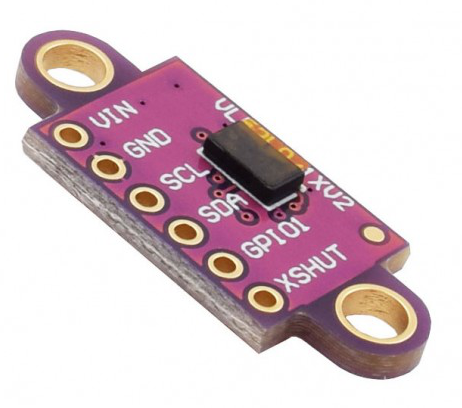
\includegraphics[width=4cm]{modulos/vl53l0x_distance_sensor.png}
\caption*{Fonte: Foto disponibilizada por botnroll}\label{wrap-fig:1}
\end{wrapfigure} 
%------------------------------------------

Os sensores de distância escolhidos para o robô foram os vl53l0x \cite{vl53l0x_datasheet}, e para fins de simplificação do circuito, foi escolhido um módulo que já tivesse um circuito pré realizado. Esse sensor consegue alcançar até dois metros de distância e é bem pequeno, por isso foi escolhido. Além disso, o sensor de inércia, que é um módulo com dois sensores que consegue agir como um acelerômetro. O módulo usado foi o Mpu-9250 \cite{MPU-9250_datasheet}. 

\begin{figure}[!ht]
    \centering
    \begin{minipage}{0.5\textwidth}
        \centering
        \caption{Protótipo Percepção Externa - PCB 2D}
        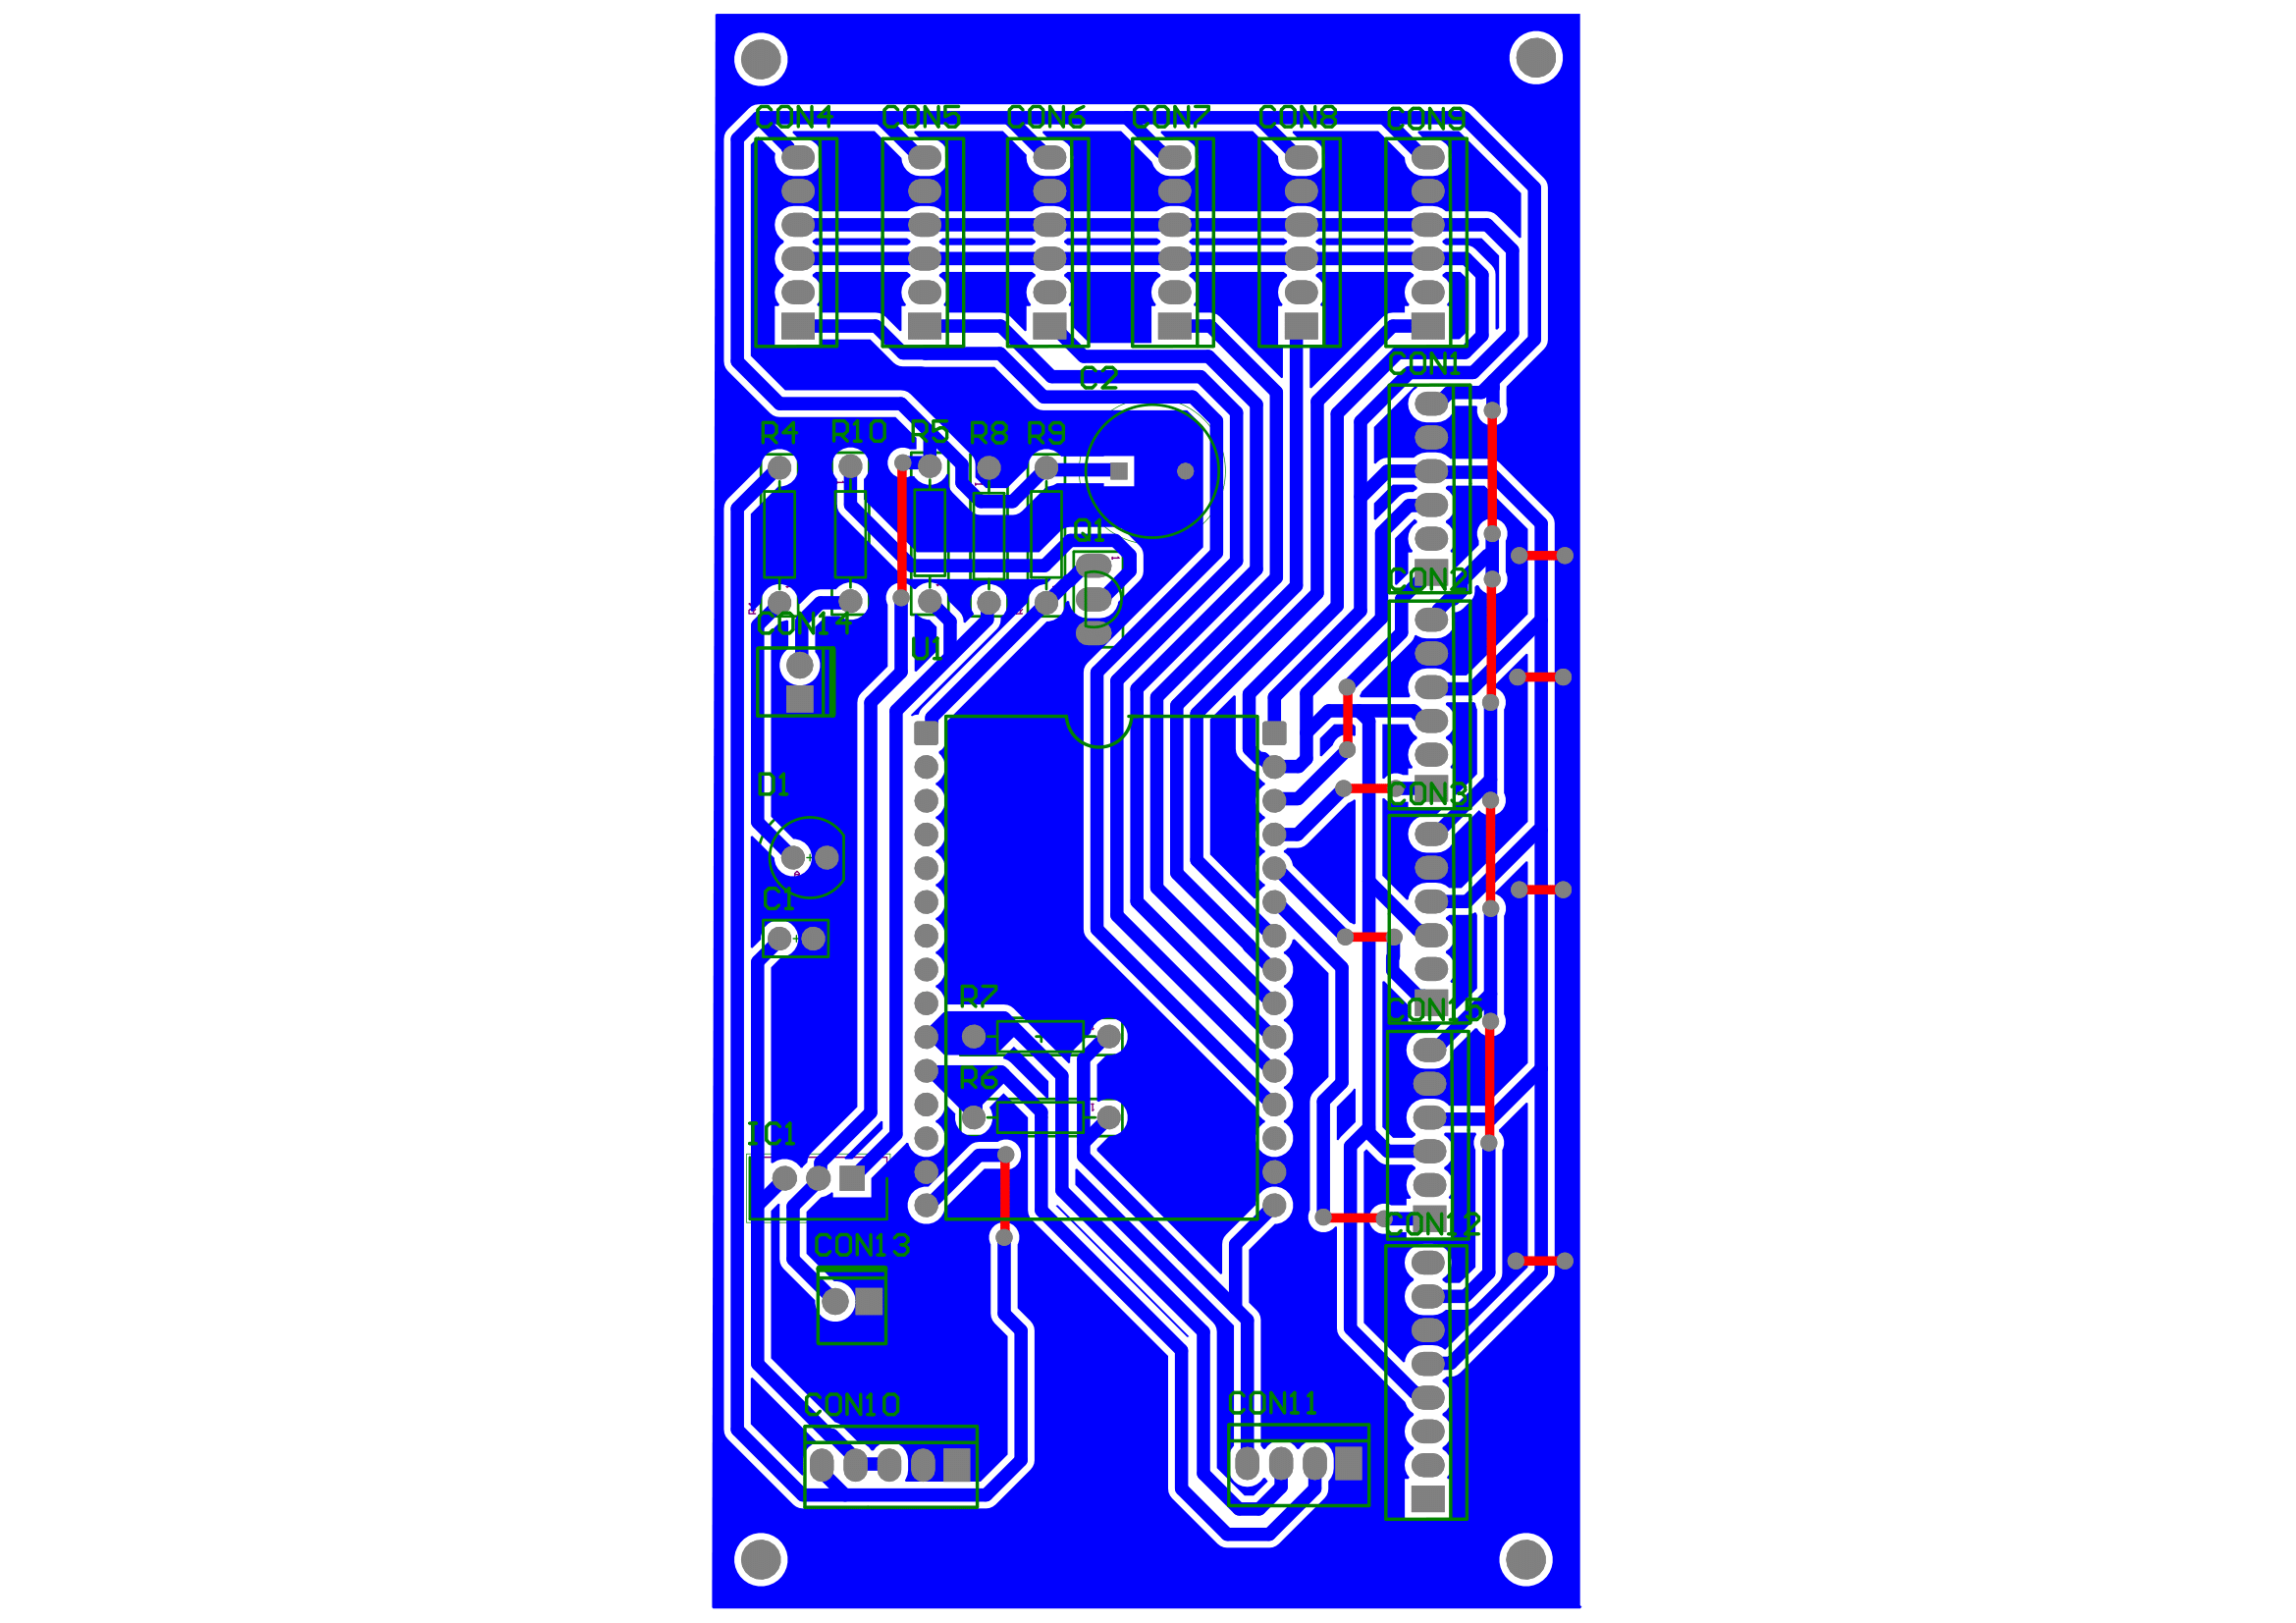
\includegraphics[width=1.03\textwidth]{modulos/Percepção_Externa-3.png} 
        \label{Protótipo Percepção Externa - PCB 2D}
    \end{minipage}\hfill
    \begin{minipage}{0.5\textwidth}
        \centering
        \caption{Protótipo Percepção Externa - PCB 3D }
        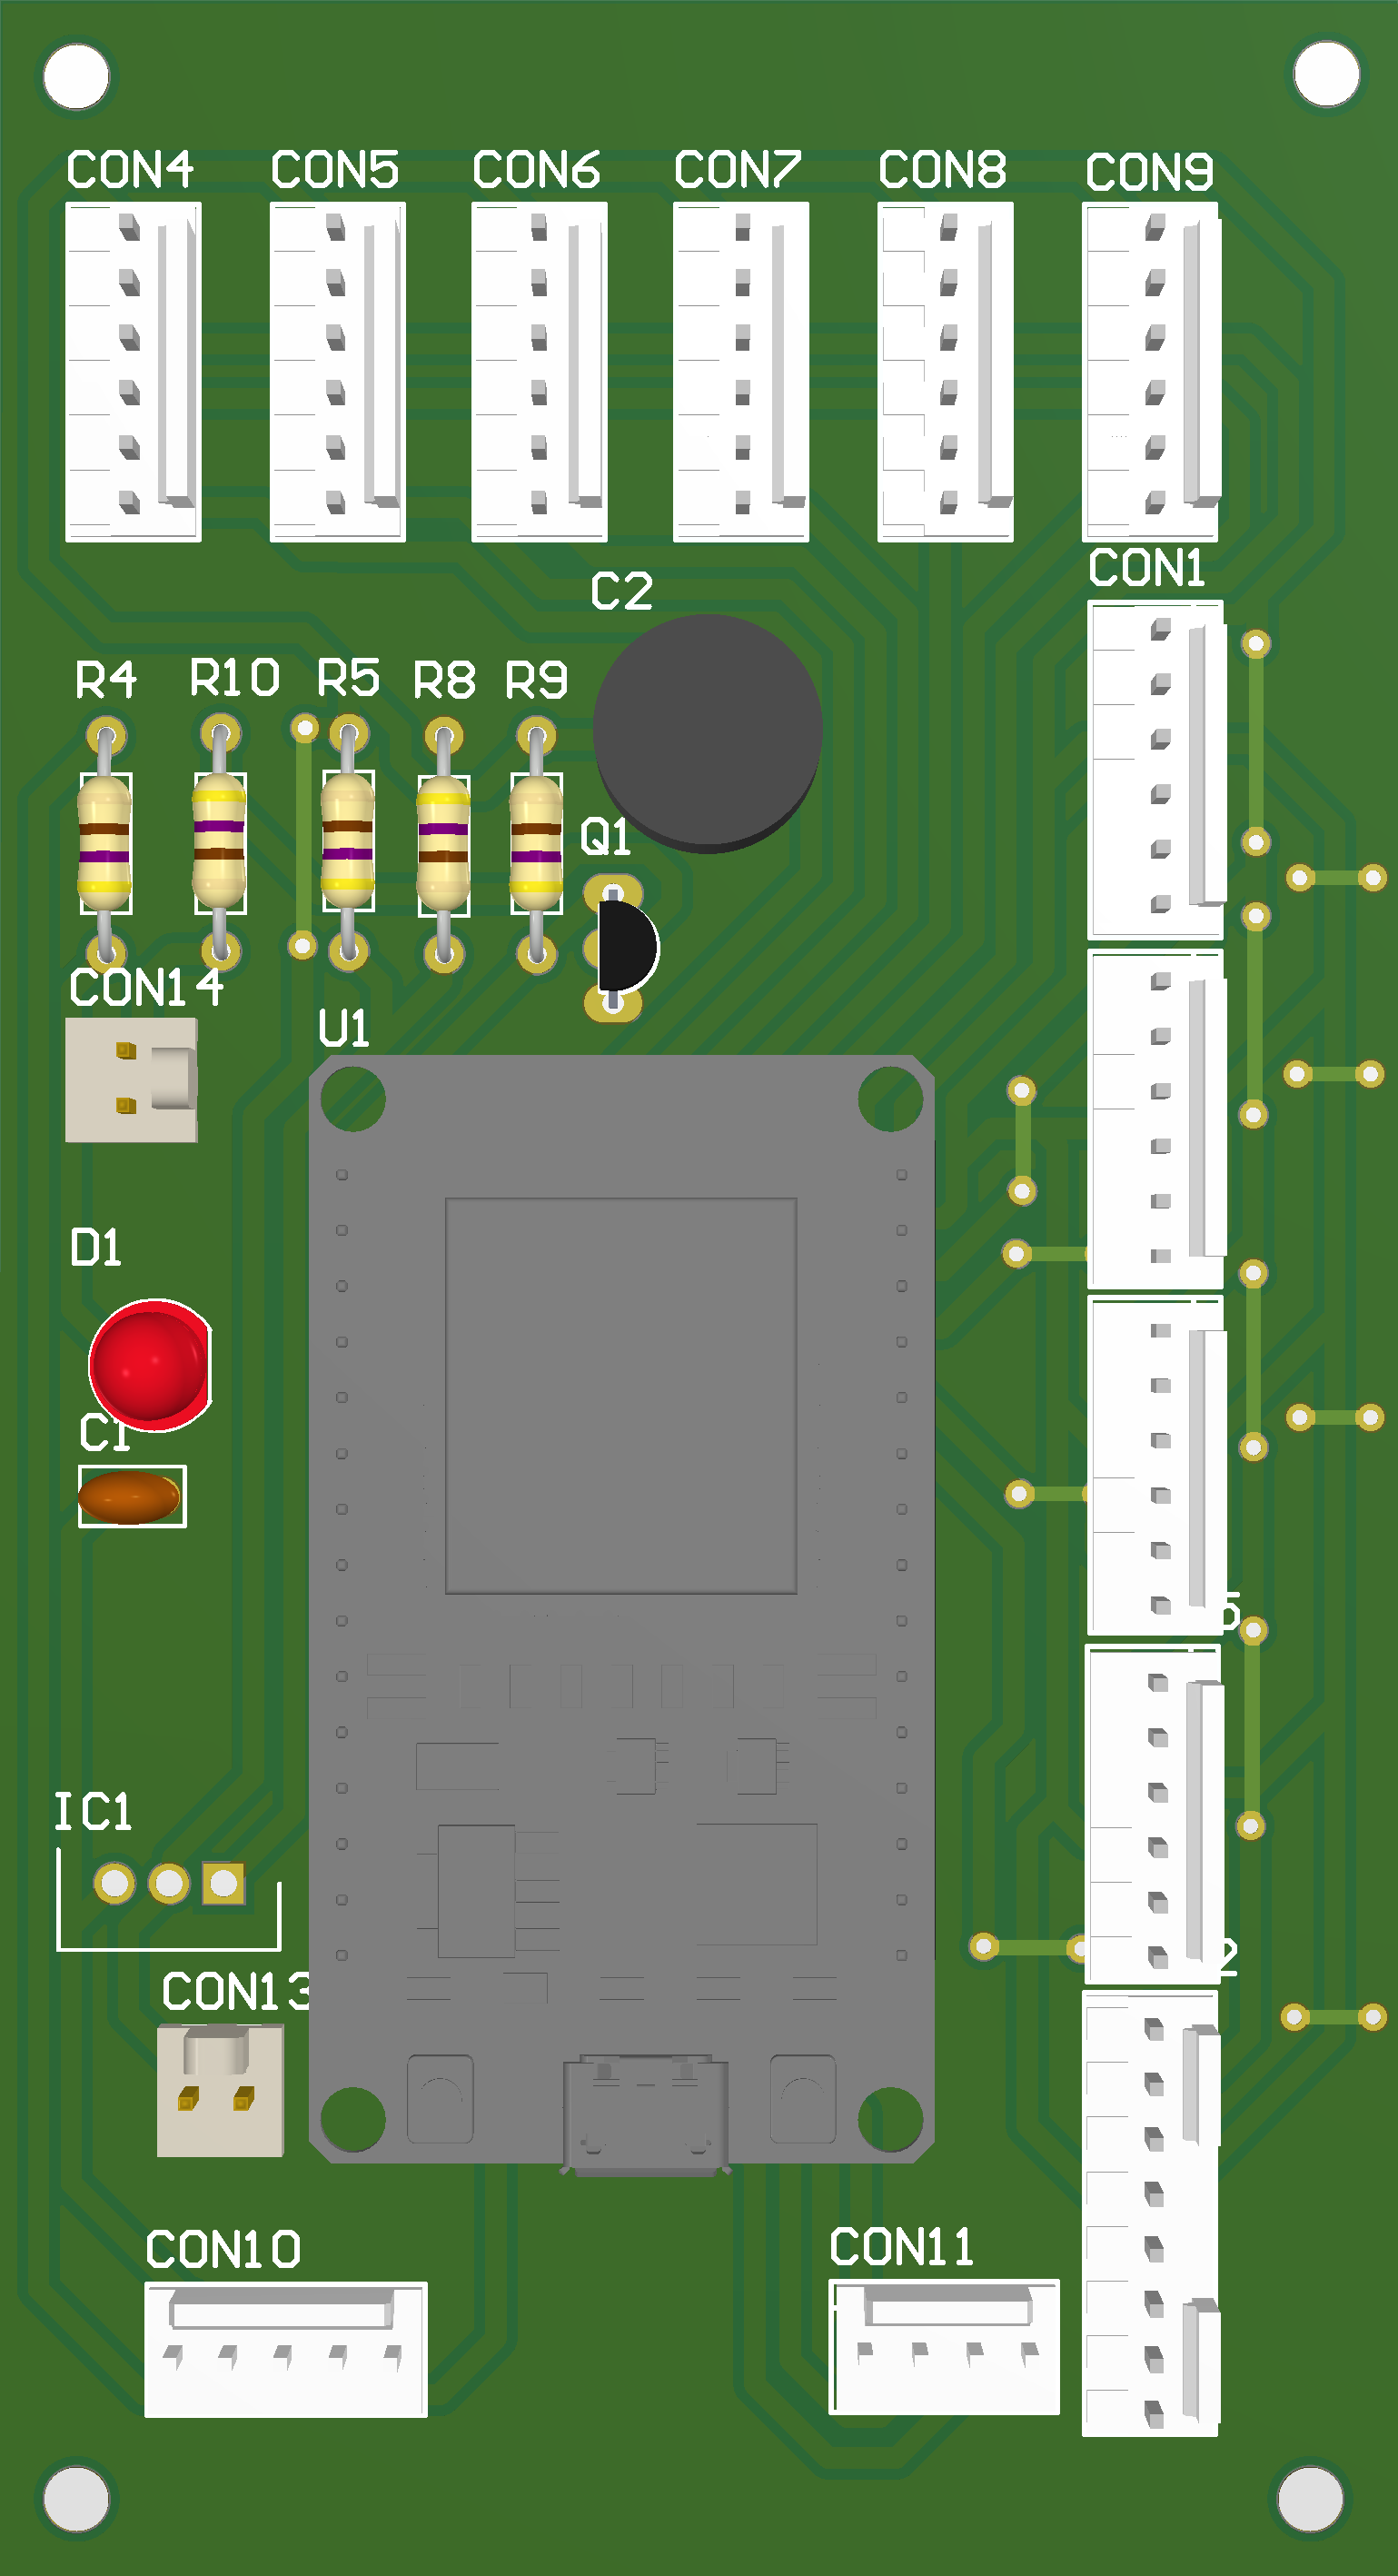
\includegraphics[width=0.4\textwidth]{modulos/Percepção_Externa.png} 
        \label{Protótipo Percepção Externa - PCB 3D}
    \end{minipage}\hfill
\caption*{Fonte: Elaborado pelo autor no software Altium Design\cite{altium21} }
\label{fig:Protótipo Percepção Externa - PCB 2D3D}
\end{figure}

  A partir do esquema elétrico que foi feito e do desenho da PCB, a placa de circuito impresso, em uma única camada (Single Layer) e dimensões de 120x60mm. As visões 2D e 3D podem ser vista na figura   ~\ref{Protótipo Percepção Externa - PCB 2D} e ~\ref{Protótipo Percepção Externa - PCB 3D}.
  
\begin{comment}
\begin{figure}[!ht]
    \centering
    \begin{minipage}{0.5\textwidth}
        \centering
        \caption{Protótipo Percepção Externa - Trilhas}
        \includegraphics[width=0.8\textwidth]{example-image-a} 
        \label{fig:figura1minipg}
    \end{minipage}\hfill
    \begin{minipage}{0.5\textwidth}
        \centering
        \caption{Protótipo Percepção Externa - Completa}
        \includegraphics[width=0.8\textwidth]{example-image-a} 
        \label{fig:figura1minipg}
    \end{minipage}\hfill
    
    \caption*{Fonte: Elaborado pelo autor }
    \label{fig:Protótipo Percepção Externa - TrilhasC}
\end{figure}
\end{comment}
%================================ PERCEPÇÂO OFICIAL ========================
\clearpage
\subsubsection{Oficial}

A placa oficial de Percepção Externa ainda não foi fabricada. Por se tratar de uma placa mais profissional, ela será mandada para ser feita para uma empresa privada ainda não escolhida, não na própria Universidade São Paulo. Assim como o protótipo, o projeto como um todo foi dividido em um esquemático e uma PCB.

\begin{figure}[!ht]
\centering
    \caption{placa de Percepção Externa - Esquemático principal }
    \centering % para centralizarmos a figura
    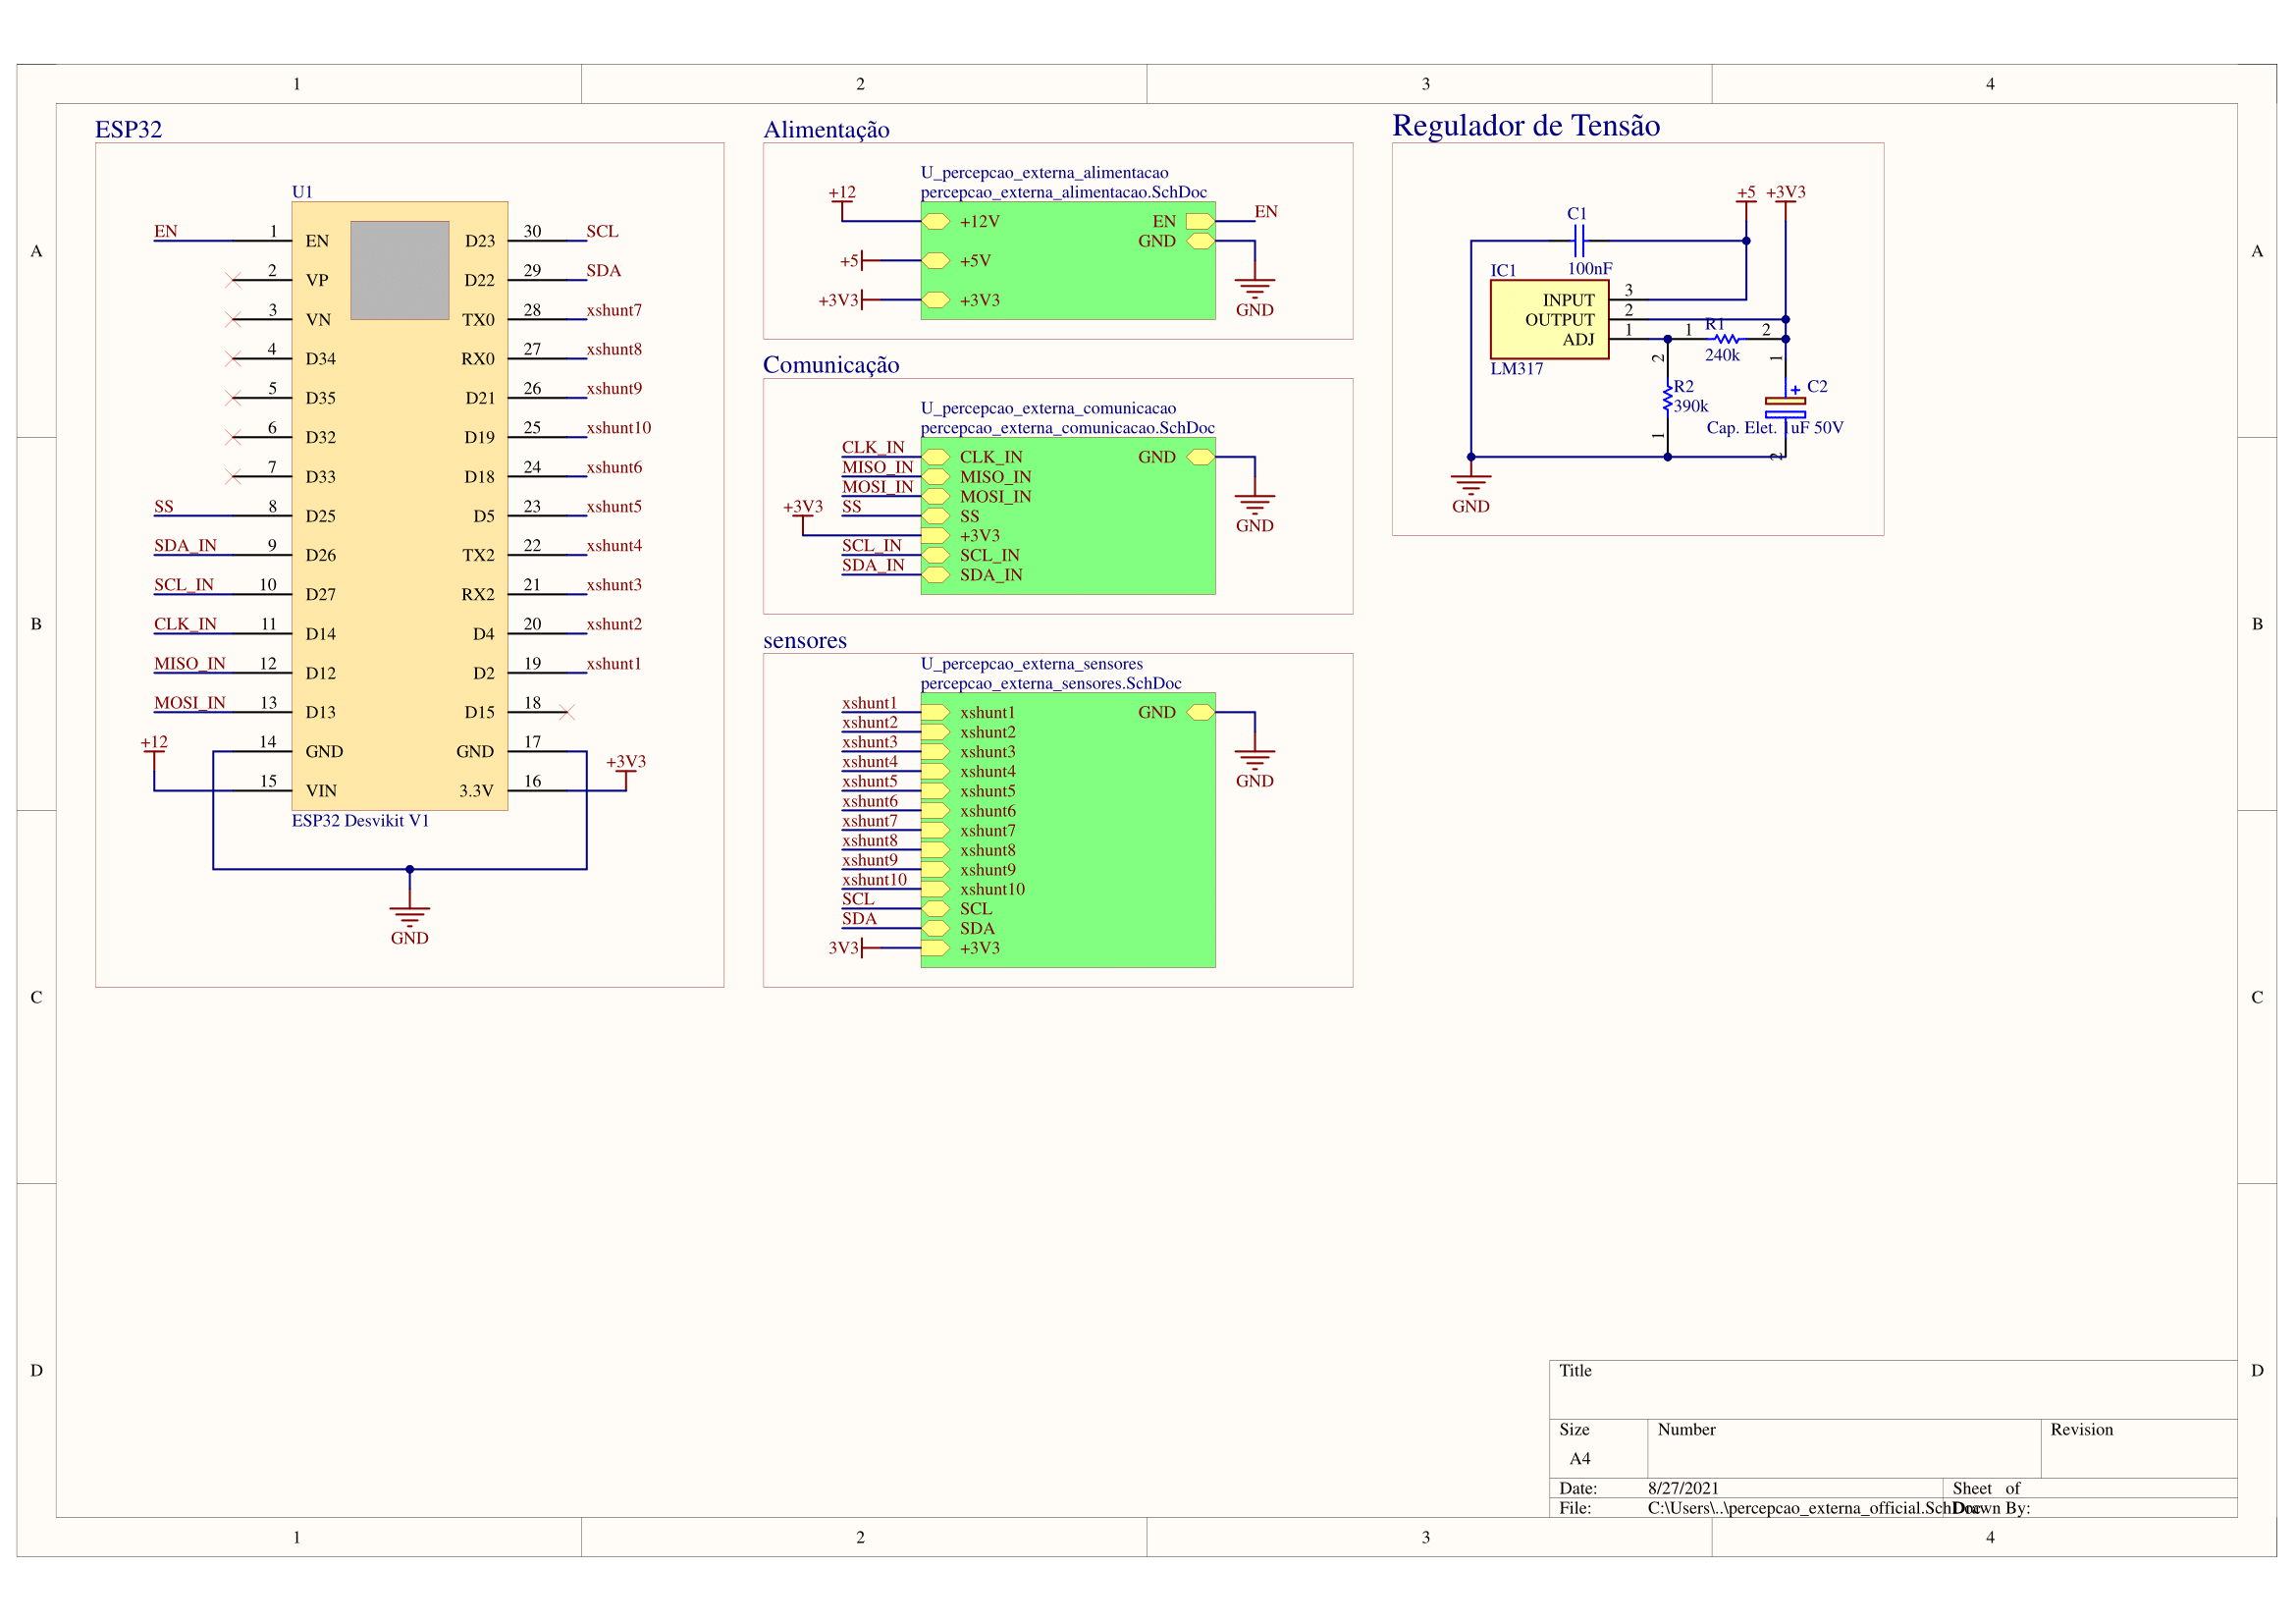
\includegraphics[width=17cm]{modulos/percepcao_externa_official-1.png}
    \caption*{Fonte: Elaborado pelo autor no software Altium Design\cite{altium21} }
    \label{Protótipo placa de ## - Esquemático principal}
\end{figure}

Para design do hardware do módulo de Percepção Externa foi utilizado o CAD e software Altium Designer 21 \cite{altium21} a partir de uma licença estudantil. O projeto completo está disponibilizado em \cite{github_modulos} e todos os componentes usado nessa versão oficial podem ser visto na tabela ~\ref{table:Componentes Utilizados na placa de Interface com Usuário}.

\begin{table}[]
\caption{Componentes Utilizados na placa de Percepção Externa}
\centering
\begin{adjustbox}{width=\columnwidth,center}
\begin{tabular}{|c|c|c|c|c|}

\hline
Component            & Description                                                    & Designator                                                                                                               & Footprint              & Quantity \\ \hline
100nF                & CAP CER DISK 10uF 50V                                          & C1                                                                                                                       & CAP CER DISK 10uF 50V  & 1        \\ \hline
Cap. Elet. 1uF   50V & Aluminum Organic   Polymer Capacitors 16volts 470uF ESR 10mohm & C2                                                                                                                       & Cap. Elet. 470uF 16V   & 1        \\ \hline
KK\_2.54\_2vias      & Conector KK 2.54mm 2   vias                                    & CON1, CON3, CON4                                                                                                         & KK\_2VIAS\_180º        & 3        \\ \hline
KK\_2.54\_6vias      & Conector KK 2.54mm 6   vias                                    & \begin{tabular}[c]{@{}l@{}}CON2, CON8, CON9,   CON10, \\ CON11, CON12, CON13, CON14, \\ CON15, CON16, CON17\end{tabular} & KK\_6vias\_180°        & 11       \\ \hline
KK\_2.54\_5vias      & Conector KK 2.54mm 5   vias                                    & CON5                                                                                                                     & KK\_5vias\_180°        & 1        \\ \hline
KK\_2.54\_4vias      & Conector KK 2.54mm 4   vias                                    & CON6                                                                                                                     & KK\_4vias\_180°        & 1        \\ \hline
KK\_2.54\_8vias      & Conector KK 2.54mm 8   vias                                    & CON7                                                                                                                     & KK\_8vias\_180°        & 1        \\ \hline
LED 3MM RED          & LED 3MM RED                                                    & D1                                                                                                                       & LED RED                & 1        \\ \hline
LM317                & Integrated Circuit                                             & IC1                                                                                                                      & TO254P467X1016X1971-3P & 1        \\ \hline
Trans BC817          & Transistor BJT NPN   BC817-25-7-F                              & Q1                                                                                                                       & SOT96P240X110-3N       & 1        \\ \hline
240k                 & RES 1206 5\%                                                   & R1                                                                                                                       & RESC3216X60N           & 1        \\ \hline
390k                 & RES 1206 5\%                                                   & R2                                                                                                                       & RESC3216X60N           & 1        \\ \hline
680R                 & Resistor                                                       & R3                                                                                                                       & RESC3216X60N           & 1        \\ \hline
2k2                  & Resistor                                                       & R4, R5                                                                                                                   & RESC3216X60N           & 2        \\ \hline
4k7                  & RES 1206 5\%                                                   & R6, R7                                                                                                                   & RESC3216X60N           & 2        \\ \hline
microcontrolador     & microcontrolador com   moculo bluethoth e wifi                 & U1                                                                                                                       & ESP32\_Desvikit\_v1    & 1        \\ \hline

\end{tabular}
\end{adjustbox}
\centering
\caption*{Fonte: Elaborado pelo autor}
\label{table:voc}
\end{table}

Em relação ao protótipo, pouco mudou da lógica por trás do circuito, a principal diferença é que o modelo oficial utiliza todos componentes com encapsulamiento SMD \cite{SMD_def} e no lugar de 6 sesnsores de distância, serão usados 10. Além disso, foi adicionado o protocolo de comunicação SPI também, como já foi comentado no início do capítulo.


A placa de circuito impresso ainda está em desenvolvimento.


\begin{comment}
%================================ PERCEPÇÂO FIRMWARE ========================
\subsection{Firmware}
\end{comment}

\end{document}